\section{Registration Protocol}\label{sec:registration_single}

\subsection{Data Structures}
\para{Topic Table}
Registrars store advertisers ads locally in a data structure called \emph{topic table}, 
indexed by advertisement topic. 
Each list of ads for a particular topic in the table  can be considered as a \emph{topic queue} because it functions like a FIFO queue.
Ads enter the queue once the registrar ticket is accepted,  and
the ad remain in the queue for a constant amount of time \texttt{target-ad-lifetime}. 
When \texttt{target-ad-lifetime} expires the ad is removed  from the queue.

\begin{figure}
    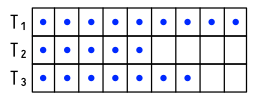
\includegraphics[width=0.35\textwidth]{img/topic-queue-diagram.png}
    \caption{Topic table structure.}
    \label{fig:topic_table}
 \end{figure}

The total size of the topic table is limited by \texttt{topic table capacity},  however there is no per-topic limits since existing number of topics in the network is unknown. 
Reasonable \texttt{topic table capacity} is 50,000 ads. 
Since ENRs are at most 300 bytes in size, these limits ensure that a full topic table consumes approximately 15MB of memory.
An advertiser can only place a single ad for a specific topic queue in the topic table at the same time; duplicate placements are rejected (although the same node may attempt placing ads for multiple topics at the same registrar).

The topic table is shared across multiple advertisers and stores topics with varying popularity (which is determined by how many nodes register the topic) among the participants of \sysname. 
It is important that the high popularity of a particular topic should not prevent peers from registering less popular topics. 
This is achieved using the waiting time function that will determine the time an advertiser will have to wait to place an ad after a ticket request,  and is detailed in Section~\ref{sec:waitingTime}.

\subsubsection{Registration Procedure}

In order to place an ad on a registrar's topic table,  the advertiser must present a valid 'ticket' to the registrar. 
%Tickets are immutable objects issued by the registrars. 
Tickets are immutable objects storing arbitrary information determined by the issuing registrar node.  While details of encoding and ticket validation are up to the implementation, tickets must contain enough information to verify that:
\begin{itemize}
    \item The advertiser attempting to use the ticket is the one which originally requested it.
    \item A ticket is valid for a single topic only.
    \item A ticket can only be used within the 'registration window' (explained below).
    \item A ticket can not be used more than once.
%     \michal{Can we enforce it? I can use the same ticket twice within the validity period, right?\onur{It seems possible for an advertiser to essentially duplicate an existing ticket by using it twice during the validity period. The duplicate ticket gets a new waiting time, accumulates a high cum. waiting time so that the advertiser can re-register its ad with significant advantage over other contenders. I think an easy fix is for registrars to drop/ignore tickets for which there is an active registration. }}
\end{itemize}

An advertiser willing to register an ad at a registrar must first obtain a ticket from that registrar by sending a 'ticket request' (TICKETREQUEST) message to the registrar. In response to the ticket request, the registrar issues an initial ticket containing a 'waiting time' and sends the ticket to the advertiser in a 'ticket response' message. The advertiser can come back to the registrar (to register an ad) after the waiting time has elapsed and present the ticket in a 'topic registration request' (i.e., REGTOPIC) message.

\michal{Change the markdown notation of variables (CAPACITY) to scientific (n)}
Any REGTOPIC messages that are not sent during the registration window determined by the waiting time (indicated in the ticket),   (as seen in Figure \ref{fig:ticket_validity}) are ignored by the registrars.  
If the advertiser comes back during the established registration window,  the advertiser can either place the ad (and notify the advertiser of a successful registration) or issue another ticket with a new waiting time in another ticket response message. 
An advertiser may be given one or more tickets in a sequence before a successful registration,  and this means that overall the advertiser waits for a 'cumulative waiting time' period that is the sum of multiple waiting times issued in each ticket in the sequence before finally registering an ad. 
Assignment of 'waiting times' is the only way the registrars can control the registrations in order to both:

\begin{itemize}
    \item Throttle ad placement rate to prevent overflowing of topic table: when the topic table is full, the advertisers must wait for already placed ads to expire first before they are allowed to register new ads.
    \item Prioritise registrations to achieve a diverse set of ads in the topic table. For example, registrations for less popular topics or registrations from advertisers that increase IP diversity (in the set of advertiser IP addresses that currently have an ad in the table) can be prioritised over others. This is useful to reduce the impact of Sybil attacks on the service discovery system.
\end{itemize}

Waiting times will be calculated according to a 'Waiting time function' detailed in Section~\ref{sec:waitingTime}.  Enforcing this time limit prevents misuse of the topic table because any topic must be important enough to outweigh the cost of waiting for ad placement. Imagine a group phone call: announcing the participants of the call using topic advertisement isn't a good use of the system because the topic exists only for a short time and will have very few participants. The waiting time prevents using the topic table for this purpose because the call might already be over before everyone could get registered. Also, it prevents attackers from overflowing topic table by regulating registrations in case of spamming attacks.

Tickets cannot be used beyond their lifetime. If an advertiser does not come back after the waiting time, all cumulative waiting time is lost and the advertiser must start over (\Cref{fig:ticket_validity}). When the ticket is issued, the node keeping it must wait until the registration window opens. The length of the registration window is implementation dependent, but by default 10 seconds is used. The ticket becomes invalid after the registration window has passed. This mechanism prevents malicious advertisers from obtaining a ticket, then just wait for a long time until a large cumulative waiting time is accumulated, and finally launch a coordinated attack to take over the topic table with their ads.

In addition to the waiting time,  the sequence of tickets issued by a registrar for a specific advertiser also records the original issue-time of the first ticket which can be used to compute the cumulative waiting time so far; that is, the time elapsed since the advertiser requested its first ticket to place its ad. The inclusion of issue-time allows the registrars to prioritise advertisers that have been waiting the most as we explain later. Because the tickets are immutable (i.e., tampering with the ticket is detectable by the registrars that originally issued the ticket), when a registrar issues a new ticket (in case a registration is not immediately successful) to an advertiser, the registrar simply copies the issue-time from the last issued ticket and use that as the issue-time of the new ticket. This means that the registrars are not required to maintain any state for each on-going ticket request given that they can simply verify the authenticity of the ticket in the incoming registration requests. 
%The registrars ensure the authenticity of the tickets they issue to the advertisers through symmetric encryption we explain below.

    
\begin{figure}
    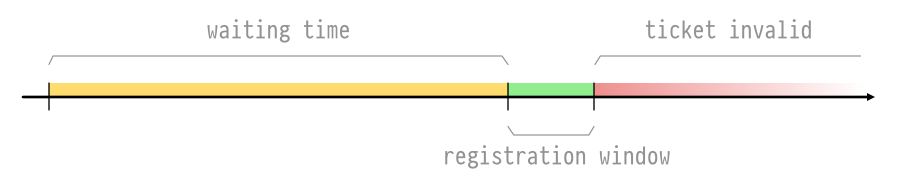
\includegraphics[width=0.5\textwidth]{img/ticket-validity}
    \caption{Ticket validity period.}
    \label{fig:ticket_validity}
\end{figure}


\michal{We're mixing here single-registrar registration process. It should be covered in the first section.}
In our approach,  advertisers start a limited number of parallel registrations in each ticket table bucket distance.
 More specifically, an advertiser follows the below steps to distribute its ads for a specific topic:
\begin{enumerate}
     %\item The advertiser (\hl{randomly?}) selects a set of K registrar nodes from each bucket distance of the ticket table structure, where the number of bucket distances (B) is a configurable parameter of the ticket table.
    \item The advertiser selects a K random of node.,  by querying the local Ethereum routing table,  for each bucket distance.
    \item A TICKETREQUEST message is initially sent to each of the selected registrar nodes in the previous step.
    \item Registrar node replies with a TICKETRESPONSE.  This message includes the TICKET which contains a waiting time and a ticket issue time.  The TICKET is stored in the table.
    \item The advertiser replies after the waiting time expires with a REGTOPIC request containing the previously received TICKET attached to it.
    \item After the TICKET reception the waiting time is calculated again at the registrar.  A registration is successful when the waiting time calculated at the registrar is smaller than the cumulative waiting time,  which means that the advertiser has waited long enough.
    \item The registrar sends a REGCONFIRMATION response to the advertiser of the successful registration. In general, the topic table occupancy is guaranteed to always remain below the topic table capacity by the waiting time calculated: the waiting time function returns increasingly large values as the topic table space runs out; the waiting time becomes infinite in case there is no space.
    \item In case the new calculated waiting time is not smaller than the cumulative waiting time, the registration is not successful and the registrar replies with a REGRESPONSE message containing a new TICKET (containing a new waiting time).
    \item A registrar gives up and stops the registration process with a registrar (say R) upon either T unsuccessful registration attempts (i.e., after being issued T tickets in REGRESPONSE messages from the registrar without a REGCONFIRMATION) or receipt of a ticket with a waiting time larger than LARGEWAIT value.  In that case,  the advertiser removes it from the ticket table and selects a new node located in the same bucket as R until filling K and the process is restarted (step 1).
    \item Similarly,  after the expiration of a previously placed ad (i.e., after the passage of ad-lifetime upon receiving a REGCONFIRMATION message) the node is removed from the ticket table and the process is restarted with a new node picked from the local table (step 1).
\end{enumerate}